\chapter{Ridge estimation of network models from time-course omics data \\ {\footnotesize(\textit{Miok, V., Wilting, S. M. and van Wieringen, W. N., Under review at Biometrical Journal})}}
\chaptermark{{\tt ragt2ridges} package}
\label{chapter:Window estimator}

\graphicspath{{Chapter4/Figs/}{Chapter4/Figs/PDF/}{Chapter4/Figs/}}%

Time-course omics experiments enable the reconstruction of the dynamics of the cellular regulatory network. Here we describe the means for this reconstruction and the downstream exploitation of the inferred network. It is assumed that one of the various vector-autoregressive (VAR) models presented here serves as a reasonably accurate description of the time-course omics data. The models are estimated through ridge penalized likelihood maximization, accompanied by functionality for the determination of optimal penalty parameters. Prior knowledge on the network topology is accommodated by the estimation procedures. Various routes that translate the fitted models into more tangible implications for the medical researcher are described. The network is inferred from the -- non-sparse -- ridge estimates through empirical Bayes probabilistic thresholding. The influence of a (trait of a) molecular entity at the current time on those at future time points is assessed by mutual information, impulse response analysis, and path decomposition of the covariance. The presented methodology is applied to the omics data from the p53 signalling pathway during HPV-induced cellular transformation. All methodology is implemented in the \texttt{ragt2ridges} package, freely available from the Comprehensive {\tt R} Archive Network.
\\
\\
This chapter corresponds to the article:\\
 Miok, V., Wilting, S. M. and van Wieringen, W. N. Ridge estimation of network models from time-course omics data \textit{Under review at Biometrical Journal}.



\section{Introduction}
The cellular regulatory system processes incoming signals. The signal usually triggers the transcription of mRNAs ultimately resulting in protein complexes executing specific tasks in response to the incoming signal. The interaction pattern of the molecular entities in the cell is described by a network. This network is often learned from observational studies that interrogated multiple, independent individuals. A powerful alternative are time-course experiments. In this type of experiment cell lines are usually manipulated by either drug treatment, ectopic gene expression or knock down and subsequently interrogated at regular intervals over time. One well known example for this is the study of cellular immortalization and transformation by (viral) oncogenes, including the human papillomavirus (HPV)-encoded E6 and E7 \cite{Band1990, Durst1987, Park1991, Pecoraro1989, Pirisi1987, Willey1991}.  The resulting sequential snapshots of the activity of each molecular entity provide insight into the dynamic aspects of the regulatory system

The goal of this paper is to illustrate how and what can be learned on the regulatory network from aforementioned time-course data. The paper starts with a description of an exemplary time-course experiment, used in the illustrations, that interrogated multiple molecular levels from multiple cell lines at various time points. It is followed by an overview of the various network analyses of these data presented here, all borrowing heavily from the field of time series analysis. The methodology underlying the first analysis is fully described in \cite{Miok2017}, but recapped here as the other analyses extend it. Next, the other network analyses, each incorporating more information through a more complex model, are presented. All models are estimated by means of ridge penalized maximum likelihood. Furthermore, downstream analysis using estimated models is discussed. Each extension is applied to the exemplary time-course experiment, using the implementation offered by the \texttt{ragt2ridges} package.


\section{Experiment}
\label{sec:experiment}
Cervical cancer is one of most frequently diagnosed cancers in women worldwide, especially in developing countries \citep{Ferlay2015}. The cancer is induced by a persistent HPV infection. Of the 150 types, about 15 are known to have oncogenic potential, of which HPV16 and HPV18 together account for around 70\% of cervical cancers. Although the majority of infected women will clear the virus, a subset will develop a persistent infection that can give rise to the development of precancerous lesions which, if left untreated, can ultimately progress into an invasive carcinoma. In vitro, this process can be mimicked by transfection of human keratinocytes with oncogenic HPV types after which four consecutive phenotypic stages of the cellular transformation are recognized: expanded lifespan, immortalization, anchorage independence and finally tumorigenicity \citep{Pirisi1987}. Previous studies \citep{Steenbergen2004, Wilting2006, Henken2007} showed that the cell line experimental model faithfully mimics cervical precancerous lesions morphologically and (epi)genetically. 

We designed an experiment involving the model system described above to enhance our molecular understanding of HPV-induced carcinogenesis. The experiment comprises four cell lines, originating from the same parental cells, of which two are affected with HPV16 and two with HPV18. Previous studies \citep{Steenbergen2004, Wilting2006, Henken2007} showed that the cell line experimental model faithfully mimics cervical precancerous lesions morphologically and (epi)genetically. During continued culturing of these cell lines abnormalities arise at the molecular level of the cells. Genomic and transcriptomic characteristics of each cell line are measured at 8 different time points. At each time point their DNA copy number, mRNA and miRNA gene expression are interrogated using oligonucleotide microarrays. 

The raw data from the cell line experiment are preprocessed as follows. The DNA copy number data are median normalized and segmented using the CBS (Circular Binary Segmentation) method \citep{Olshen2004}. The mRNA gene expression data are RMA background corrected \citep{Irizarry2003}, between-array normalized by the robust quantile method \citep{Boldstad2003}, and finally transformed using a variance stabilizing transformation \citep{Huber2002}. The miRNA gene expression data are preprocessed similarly, but without the background correction. 

For the illustration of the exposed methodology and software the data are limited to that related to the p53 signaling pathway, known to be directly altered in this model system by the viral oncogene E6. The mRNA gene expression data are limited to the genes that map to the p53 signaling pathway as defined by the KEGG repository \citep{Kanehisa2000}. Based on the chromosomal location DNA copy number transcripts are matched to the mRNA expression features (employing the {\tt overlapPlus} matching procedure of the \texttt{sigaR} package, \citealp{Wieringen2012}). The miRNA transcripts are a selection on the basis of temporal differential expression (determined using the method of \citealp{Miok2014}), that are either up- or down-regulated in at least 3 out of 4 cell lines. Both mRNA gene expression and DNA copy number data then comprise $p=64$ genes, while the miRNA gene expression data  includes $q=106$ genes, all measured at $\mathcal{T}=8$ time points in $n=4$ cell lines. In the third cell line the miRNA expression hybridizations of the fourth and fifth time point failed and corresponding array columns contain missings. These (P53 signalling pathway related mRNA, miRNA, and DNA copy number) data are included in the R-package {\tt ragt2ridges}. 

\section{Methods}
Experiments like the one described above may provide insight into the temporal and contemporaneous relations among molecular entities of (say) the P53 signaling pathway. The temporal relations reflect the conditional (in)dependency between two molecular entities at consecutive time points ($t$ and $t+1$) given all others at time $t$. On the other hand, contemporaneous relations reflect the conditional in/dependency between two molecular entities at the same point given all others at the same time point \textit{and} all (!) at the preceding time point. These relations are aggregated in the time-series chain graph \citep{Dahlhaus2000}. To shed light on such graphs several multivariate statistical techniques, all based on the vector auto-regressive (VAR) processes and each answering a different question, are proposed:

\begin{compactitem}
\item The first technique aims to unravel the dynamic interrelatedness of the variates (e.g. mRNA genes) of a single molecular level (e.g. mRNA gene expression). To this end a VAR(1) model is assumed to describe the time-series data from this molecular level. The model explains the gene expression at the present time by that of the one (hence, the '1' in VAR(1) model) time point directly preceding it. The model thus explicates the temporal dependencies among the genes, but also captures the contemporaneous ones (through the inverse of the error covariance matrix). The top left panel of Figure \ref{fig:VARmodels} provides an illustration of the network of temporal and contemporaneous interactions among three genes as implicated by a VAR(1) model. 

\item The previous technique is extended to assess the presence of dynamic dependencies over a longer time range than that implied by the VAR(1) model. This is done through the VAR(2) model, which includes an additional explanatory time point, i.e. the two time points directly preceding the current one may both contribute to the observed variation in the latter. The top right panel of Figure \ref{fig:VARmodels} illustrates the temporal and contemporaneous relations among the variates captured by a VAR(2) model. 

\item When cell lines can be divided into groups (e.g. in the aforementioned experiment by the HPV type by which they have been transfected), differences among the groups' interaction networks may be identified. Hereto a group-wise VAR(1) model is assumed but fitted jointly to facilitate the borrowing of information when they share network features. The result of this approach is depicted in the right bottom panel of Figure \ref{fig:VARmodels}.



\item When information on additional molecular levels (e.g. DNA copy number or microRNA gene expression) is available, those levels may be incorporated into the network. The VARX(1) model integrates time-varying covariates from other molecular levels (corresponding the `X' in VARX) into the VAR(1) model. The network of this VAR(1) extension to include exogenous data is illustrated in bottom left panel Figure \ref{fig:VARmodels}.



\begin{figure}[h!]
\centering
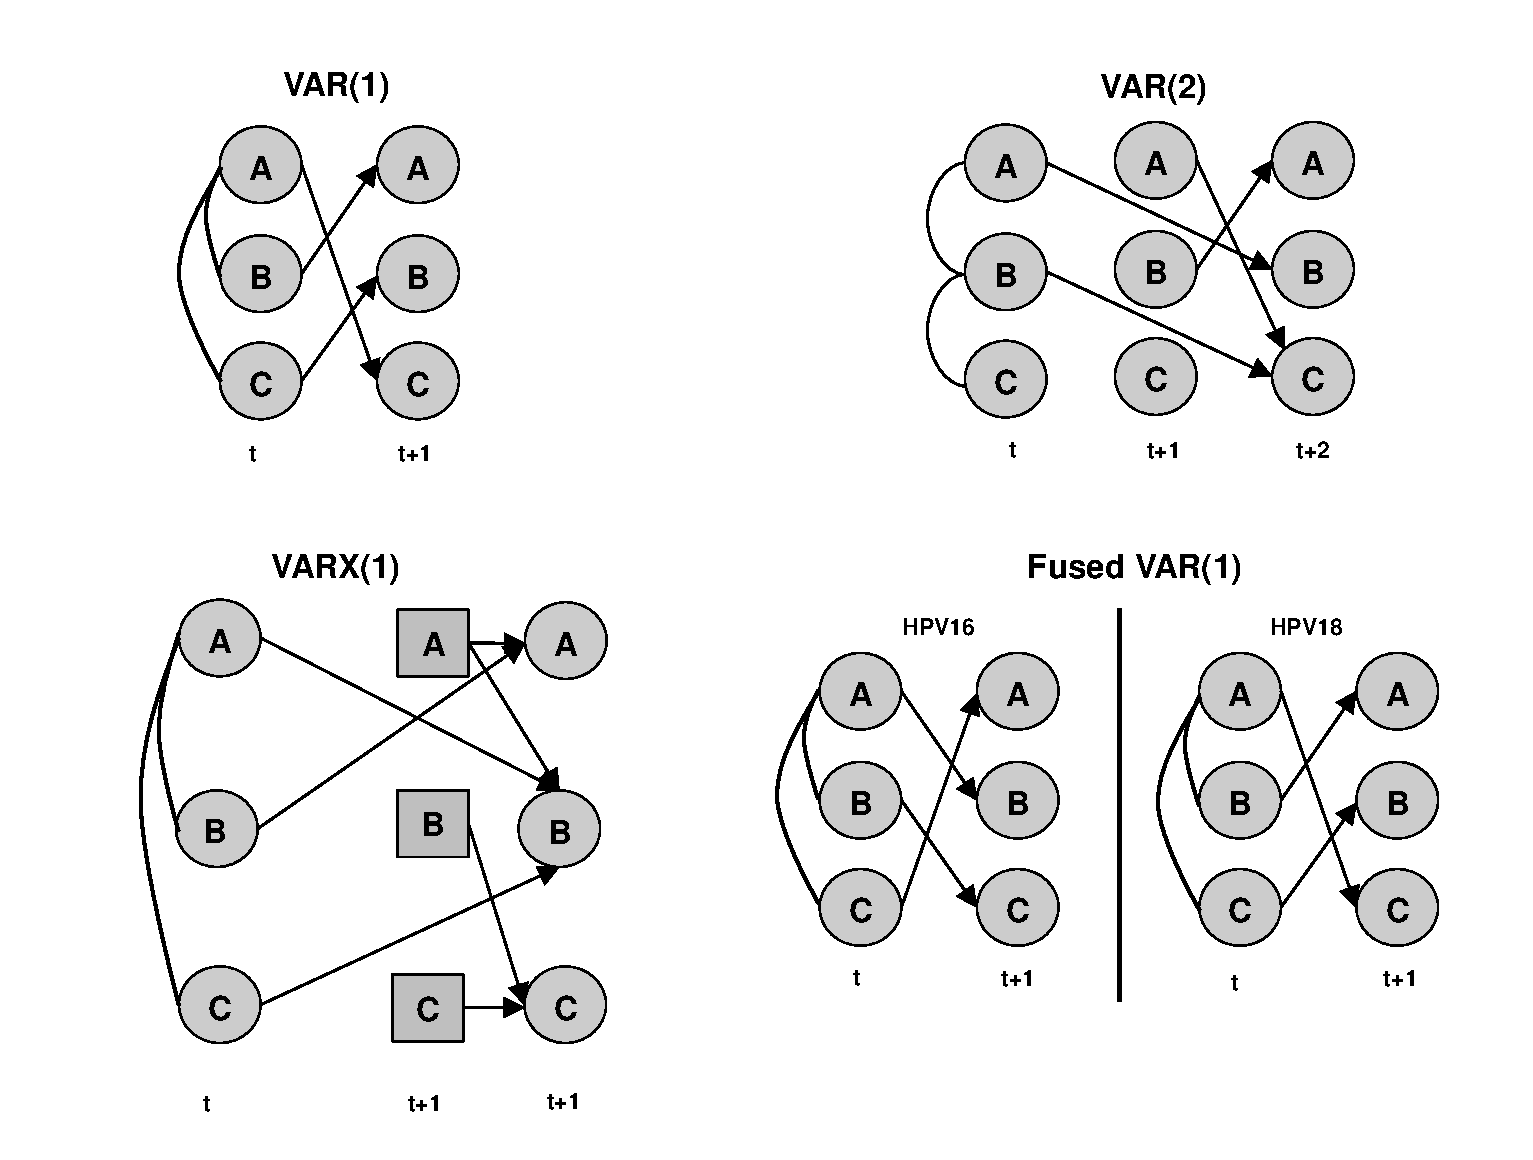
\includegraphics[scale=0.6]{Figure_2.eps}
\caption{Illustration of the time-series chain graphs underlying the various vector autoregressive models. Circles represents the endogenous molecular entities A, B and C (e.g., mRNA expression of genes) at various time points. Squares represent time-varying covariates (e.g., DNA copy number and miRNA expression). Arrows and lines indicate the temporal and contemporaneous (respectively) relations among the molecular entities. The various panels (starting top left and going clock-wise) illustrate the time-series chain graphs of the VAR(1), VAR(2), multi-group VAR(1) and VAR1(X) models.}
\label{fig:VARmodels}  
\end{figure}
\end{compactitem}
The models described above are estimated from high-dimensional data through ridge penalized, full likelihood maximization. Resulting estimates are sparsified post-estimation to arrive at a network comprising the main edges. Further methodology exploits the estimated models in order the answer additional biological questions. 



\section{The VAR(1) model}
Knowledge of the dynamic cellular regulatory patterns may enhance the understanding of cervical carcinogenesis. Hereto temporal and contemporaneous gene-gene interactions need to be identified from the HPV-cell lines data. This is facilitated by the methodology presented in \cite{Miok2017}, which also describes how inferred model and graph may be exploited to deduce tangible implications for the medical researcher. Here this is briefly recapitulated. We  refer to \cite{Miok2017} for the illustration of the VAR(1) model estimation and its down-stream exploitation on the P53 signalling pathway mRNA gene expression data of the cervical cancer time-course experiment. 


Let $\mathbf{Y}_{*,t,i}$ be a random vector representing the $p$-dimensional mRNA gene expression data of sample $i$ $(i=1,\hdots,n)$ at time point $t$ $(t=1,\hdots,\mathcal{T})$. These data are assumed to follow a VAR(1) process, where the data at the current time point $t$ are explained by that at the previous time point $t-1$. In vector form the VAR(1) model is: $\mathbf{Y}_{*,t,i}  = \boldsymbol{\nu} + \mathbf{A} \mathbf{Y}_{*,t-1,i} + \boldsymbol{\varepsilon}_{*,t,i}$, where $\boldsymbol{\nu}$ is the intercept vector assumed to be zero (i.e. $\boldsymbol{0}_{p}$), $\mathbf{A}$ is the $p \times p$-dimensional matrix of auto-regression coefficients, and $\boldsymbol{\varepsilon}_{*,t,i}$ the errors which are independently and identically distributed in accordance with a $\mathcal{N}(\boldsymbol{0}_{p}, \boldsymbol{\Omega}_{\varepsilon}^{-1})$ law. For more details about the model see \cite{Lutkepohl2005, Hamilton1994}.

Parameters of the VAR(1) model are obtained from the ridge penalized maximum likelihood (ML) estimation. The likelihood, using $\mathbf{Y}_{*,t,i}|\mathbf{Y}_{*,t-1,i}\sim\mathcal{N}(\mathbf{A}\mathbf{Y}_{*,t-1,i},\mathbf{\Omega}_{\varepsilon}^{-1})$, is $L(\mathbf{Y}; \mathbf{A}, \boldsymbol{\Omega}_{\varepsilon}) = \prod_{i=1}^n \prod_{t=2}^{\mathcal{T}}P(\mathbf{Y}_{*,t,i}|\mathbf{Y}_{*,t-1,i})$. To address the high-dimensionality of the data its logarithm is augmented with ridge penalties on the $\mathbf{A}$ and $\mathbf{\Omega}_{\varepsilon}$ parameters: $\tfrac{1}{2} \lambda_a n(\mathcal{T}-1) \| \mathbf{A} - \mathbf{A}_0 \|_F^2$ and $\tfrac{1}{2} \lambda_{\omega} n(\mathcal{T}-1) \| \mathbf{\Omega}_{\varepsilon} - \mathbf{\Omega}_0 \|_F^2$, respectively. In this $\lambda_a$ and $\lambda_{\omega}$ are penalty parameters, matrices $\mathbf{A}_0$ and $\boldsymbol{\Omega}_0$ are user-specified target matrices towards the parameters are shrunken for large values of the penalty parameters, and $\| \cdot \|_F$ denotes the Frobenius norm. 


The estimators of the VAR(1) model parameters $\mathbf{A}$ and $\boldsymbol{\Omega}_{\varepsilon}$ are obtained through ridge penalized log-likelihood maximization (see \cite{Miok2017} for details). The estimator of autoregression parameters $\mathbf{A}$ (fixing $\boldsymbol{\Omega}_{\varepsilon}$) is: 
\begin{eqnarray}\label{ridgeA1}
\mbox{vec}[ \hat{\mathbf{A}}(\lambda_a) ] & = &  [\lambda_a \mathbf{I}_{p^2 \times p^2}  + \hat{\boldsymbol{\Gamma}}(0) \otimes \mathbf{\Omega}_{\varepsilon} \big) ]^{-1} \times \, \{ \lambda_a \mbox{vec}(\mathbf{A}_0) + \mbox{vec} [\mathbf{\Omega}_{\varepsilon} \hat{\boldsymbol{\Gamma}}(-1) ] \},
\end{eqnarray}
where $\hat{\boldsymbol{\Gamma}}(0) = \frac{1}{n(\mathcal{T}-1)} \sum_{i=1}^{n}\sum_{t=2}^{\mathcal{T}} \mathbf{Y}_{*,t-1,i} \mathbf{Y}_{*,t-1,i}^{\top}$ and \\
$\hat{\boldsymbol{\Gamma}}(-1) = \frac{1}{n(\mathcal{T}-1)} \sum_{i=1}^{n} \sum_{t=2}^{\mathcal{T}} \mathbf{Y}_{*,t,i} \mathbf{Y}_{*,t-1,i}^{\top}$. The error precision matrix estimator, for fixed $\mathbf{A}$, is (cf. \cite{Wieringen2016}): 
\begin{eqnarray} \label{ridgePrecision}
\widehat{\mathbf{\Omega}}_{\varepsilon} (\lambda_{\omega}) & = & \{ [ \lambda_{\omega} \mathbf{I}_{p \times p} + \tfrac{1}{4} (\mathbf{S}_{\varepsilon} - \lambda_{\omega} \mathbf{\Omega}_0)^2 ]^{1/2} +
\tfrac{1}{2} (\mathbf{S}_{\varepsilon} - \lambda_{\omega} \mathbf{\Omega}_0) \}^{-1},
\end{eqnarray}
where $\mathbf{S}_{\varepsilon}$ is the sample covariance matrix of the errors:
\begin{eqnarray*}
\mathbf{S}_{\varepsilon} & = & \frac{1}{n(\mathcal{T}-2)}\sum_{i=1}^{n} \sum_{t=2}^{\mathcal{T}} \left[\mathbf{Y}_{*,t,i} - \mathbf{A} \mathbf{Y}_{*,t-1,i} \right] \left[\mathbf{Y}_{*,t,i} - \mathbf{A} \mathbf{Y}_{*,t-1,i} \right]^{\top}.
\end{eqnarray*}
The final estimators of $\mathbf{A}$ and $\boldsymbol{\Omega}_{\varepsilon}$ result from an iterative procedure which alternates between the updating of one estimator while keeping the other fixed, until convergence. The procedure is initiated with the ridge least squares estimator of $\mathbf{A}$, which does not involve $\boldsymbol{\Omega}_{\varepsilon}$. In this penalty parameters $\lambda_a$ and $\lambda_{\omega}$ are chosen to maximize the leave-one-out cross-validated (LOOCV) log-likelihood. 

Prior to the parameter estimation, the penalty parameters $\lambda_a$ and $\lambda_{\omega}$ are chosen through LOOCV log-likelihood maximization. The convergence of this optimization procedure may be inspected visually by contourplots. With optimal penalty parameters at hand, the (penalized) estimates of $\mathbf{A}$ and $\boldsymbol{\Omega}_{\varepsilon}$ are obtained. 

The resulting ridge estimates of $\mathbf{A}$ and $\mathbf{\Omega}_{\varepsilon}$ are not sparse. For many practical purposes, however, this is desirable. To this end their support may be inferred  by means of various  post-estimation thresholding procedures. Minimally sophisticated choices would be: \textit{1)} thresholding on the absolute values of the matrix entries, and \textit{2)} selection of the top absolute values of $\mathbf{A}$. A third procedure with a more probabilistic flavour employs the empirical Bayes approach of \cite{Efron2004} and implemented by \cite{Strimmer2008}), which yields the probability of an edge being ``interesting'' given its observed edge strength (i.e., a statistic derived from the parameter estimates, cf. \cite{Miok2017}, Section 4).
 
The inferred support does not -- strictly -- match with the non-sparse parameter estimates. To align those two the VAR(1) model is re-fitted. To this end penalty parameters need to be re-determined, now accommodating the inferred support of the VAR(1) model parameters. As the optimal penalty parameters are likely to be smaller, this will yield less biased estimates. With re-determined penalty parameters the final estimate of the VAR(1) model parameters are obtained. The final VAR(1) model is visualized as a time-series chain graph depicting all temporal and contemporaneous relations (see Figure 1 of \cite{Miok2017}).

To facilitate the understanding of the (mRNA expression) dynamics implied by the fitted VAR(1) model \citep{Miok2017} present several downstream analyses. A first step in this direction is impulse response analysis, which evaluates the effect of a change in the error at one time point on the variates at a future time point. For the VAR(1) model this change, operationalized as the derivative of $Y_{*, i, t+\tau}$ with respect to $\varepsilon_{*, i, t}$, amounts to $\mathbf{A}^{\tau}$ \citep{Hamilton1994}. This may be helpful when designing knock-out experiments. Alternatively, mutual information analysis yields a (generalized) correlation measure between the variate at one time point and the variates at a future time point. The mutual information of the VAR(1) model is:
\begin{eqnarray*}
\mathcal{I}(\mathbf{Y}_{*,t+\tau,i},Y_{j,t,i}|\mathbf{Y}_{*,t-1,i},\mathbf{Y}_{*,t-2,i}) & = & \log \{ |\mbox{Var}(\mathbf{Y}_{*,t+\tau,i}|\mathbf{Y}_{*,t-1,i},\mathbf{Y}_{*,t-2,i}) | \}-  
\\
& & \log \{ | \mbox{Var}(\mathbf{Y}_{*,t+\tau,i}|Y_{j,t,i},\mathbf{Y}_{*,t-1,i},\mathbf{Y}_{*,t-2,i}) | \}.
\end{eqnarray*}
This measure aids in the identification of the most influential nodes.


With re-estimated model parameters and the inferred network at hand, node statistics can be calculated: various network measures, e.g. degree, centrality (see \cite{Newman2010}), mutual information, and impulse response. Table 1 of \cite{Miok2017} presents these for the most interesting genes from the P53 signaling pathway model, defined by a large number of out- and in-degree edges and, henceforth, for convenience referred to as `regulators' and `regulatees' genes, respectively. For these genes centrality measures, mutual information and impulse response are given. The centrality measures are indeed high for `regulators', which corroborates with it intuitively understood by an influential node.

Finally, path decomposition analysis unravels the association between two nodes at different time points in terms of the paths connecting them. Hereto the covariance between $Y_{j_1,t,i}$ and $Y_{j_2,t+\tau,i}$ for $\tau\ge 0$ can be decomposed as a sum over all paths connecting $j_1$ and $j_2$ in the time-series chain graph \citep{Miok2017}:
\begin{eqnarray*}
\mbox{Cov}(Y_{j_1,t,i},Y_{j_2,t+\tau,i}|\mathbf{Y}_{*,t-1,i}) \, \, \, = \, \, \, (\mathbf{\Sigma}_{\varepsilon} \mathbf{A}^{\tau})_{j_1,j_2}\, \, \, = \, \, \,\sum_{j'=1}^p (\mathbf{\Sigma}_{\varepsilon})_{j_1,j'} (\mathbf{A}^{\tau})_{j',j_2},
\end{eqnarray*}
where $(\mathbf{\Sigma}_{\varepsilon})_{j_1,j'}$ can be further decomposed in terms of the contemporaneous paths connecting $j_1$ and $j'$ (see \cite{Jones2005}). As such it guides in the search for the most important paths by which a molecular signal travels between these two nodes. 


\section{The VAR(2) model}
The VAR(1) model uses only information of the last time point to explain that of the next. The dynamics may, however, extend over more than two time points. That is, an additional explanatory time point may yield a significantly better fit. This can be assessed using a VAR(2) model, which includes an extra historical time point to explain the variation in the present. The VAR(2) model, where the `2' again refers to the lag in the explanatory part of the model, is:
\begin{eqnarray*}
\mathbf{Y}_{*,t,i}  & = & \boldsymbol{\nu} + \mathbf{A}_1 \mathbf{Y}_{*,t-1,i} + \mathbf{A}_2 \mathbf{Y}_{*,t-2,i} + \boldsymbol{\varepsilon}_{*,t,i},
\end{eqnarray*}
in which $\mathbf{Y}_{*,t,i}$, $\boldsymbol{\nu}$ and $\boldsymbol{\varepsilon}_{*,t,i}$, endowed with an identical and independent normal distributional assumption: $\boldsymbol{\varepsilon}_{*,t,i} \sim \mathcal{N}( \mathbf{0}_{p}, \mathbf{\Sigma}_{\varepsilon})$ (as for the VAR(1) model). The parameters $\mathbf{A}_1$ and $\mathbf{A}_2$ are the lag one and two auto-regression coefficient matrices, respectively. Finally, as for the VAR(1) model, we assume that (after centering) $\boldsymbol{\nu} = \mathbf{0}_{p}$. The VAR(2) model is often rewritten in the form of a VAR(1) model:
\begin{eqnarray} \label{form:VAR2asVAR1}
\left(\begin{array}{l} \mathbf{Y}_{*,t,i} \\ \mathbf{Y}_{*,t-1,i}  \end{array} \right) & = & \left( \begin{array}{ll} \mathbf{A}_1 & \mathbf{A}_2 \\ \mathbf{I}_{pp} & \mathbf{0}_{pp} \end{array} \right) \left( \begin{array}{l} \mathbf{Y}_{*,t-1,i} \\ \mathbf{Y}_{*,t-2,i}  \end{array} \right) + \left( \begin{array}{l}  \boldsymbol{\varepsilon}_{*,t,i}
\\ \mathbf{0}_{p} \end{array} \right).
\end{eqnarray}
More condensed, this amounts to $\mathbf{Z}_{*,t,i}  =  \mathbf{C} \mathbf{Z}_{*,t-1,i} +  \tilde{\boldsymbol{\varepsilon}}_{*,t,i}$, 
with definitions of its constituents straightforwardly deduceable from Equation (\ref{form:VAR2asVAR1}). The error precision matrix of the rewritten model, denoted $\tilde{\mathbf{\Omega}}_{\varepsilon}$, is a $2\times 2$ block matrix matrix with the left upper block equal to $\mathbf{\Sigma}_{\varepsilon}^{-1}$ with the other blocks all equalling $\mathbf{0}_{p \times p}$. This precision matrix is degenerated -- as it is not strictly positive definite -- but is defined here only for the derivation of the parameter estimators.

The parameters of the VAR(2) model are estimated by means of a ridge ML procedure. Using the Markov property implied by the VAR(2) model, the likelihood is:
\begin{eqnarray*}
L(\mathbf{Y}; \mathbf{A}_1, \mathbf{A}_2, \boldsymbol{\Sigma}_{\varepsilon}) & = & \prod_{i=1}^n \prod_{t=3}^{\mathcal{T}}P(\mathbf{Y}_{*,t,i}|\mathbf{Y}_{*,t-1,i},\mathbf{Y}_{*,t-2,i}).
\end{eqnarray*}
The normal assumption on the error enables the likelihood to be expressed explicitly in terms of the VAR(2) model parameters. Take the logarithm and augment the result with the ridge penalty $\lambda_{a,1} \| \mathbf{A}_1 - \mathbf{A}_{1,0} \|_2^2 + \lambda_{a,2} \| \mathbf{A}_2 - \mathbf{A}_{2,0} \|_2^2 + \lambda_{\omega} \| \mathbf{\Omega}_{\varepsilon} - \mathbf{\Omega}_{0} \|_2^2$. The first two summands of the penalty are written as $\mbox{tr}\{ [ \mbox{vec}(\mathbf{C}) - \mbox{vec}(\mathbf{C}_0)]^{\top} \mathbf{\Lambda}_a [ \mbox{vec}(\mathbf{C}) - \mbox{vec}(\mathbf{C}_0)] \}$ in which $\mathbf{\Lambda}_a$ a $4p^2 \times 4p^2$ dimensional, diagonal matrix with $(\mathbf{\Lambda}_a)_{jj} = \lambda_{a,1}$ for $j=1,\ldots, 2p^2$ and $(\mathbf{\Lambda}_a)_{jj} = \lambda_{a,2}$ for $j=2p^2 +1,\ldots, 4p^2$. This gives the penalized log-likelihood. To obtain the estimator of $\mathbf{C}$ (and thereby $\mathbf{A}_1$ and $\mathbf{A}_2$), equate the derivative of the penalized log-likelihood with respect to $\mathbf{C}$ to zero. Solving the resulting estimating equation gives the ridge ML estimator:
\begin{eqnarray*}
\textrm{vec} \big[\widehat{\mathbf{C}}(\boldsymbol{\Lambda}_a) \big] & = & \big[\boldsymbol{\Lambda}_a + \widehat{\boldsymbol{\Gamma}}_{zz}(0) \otimes\tilde{\boldsymbol{\Omega}}_{\varepsilon} \big]^{-1}
\big\{ \boldsymbol{\Lambda}_a \textrm{vec}(\mathbf{C}_0)+\textrm{vec} \big[ \tilde{\boldsymbol{\Omega}}_{\varepsilon} \widehat{\boldsymbol{\Gamma}}_{zz}(-1)\big] \big\},
\end{eqnarray*}
where $\widehat{\boldsymbol{\Gamma}}_{zz} (0) = \frac{1}{n(\mathcal{T}-2)} \sum_{i=1}^{n} \sum_{t=3}^{\mathcal{T}} \mathbf{Z}_{*,t-1,i} \mathbf{Z}_{*,t-1,i}^{\top}$ and \\
 $\widehat{\boldsymbol{\Gamma}}_{zz}(-1) = \frac{1}{n (\mathcal{T}-2) } \sum_{i=1}^{n} \sum_{t=3}^{\mathcal{T}} \mathbf{Z}_{*,t,i}\mathbf{Z}_{*,t-1,i}^{\top}$. 

To ensure that the bottom left and right $p \times p$ dimensional blocks of the matrix $\mathbf{C}$ are indeed $\mathbf{I}_{pp}$ and $\mathbf{0}_{pp}$ we impose linear equality constraints on corresponding elements of $\mathbf{C}$. Let the linear equality constraints on $\mathbf{C}$ be given by $\mathbf{Q} \textrm{vec}(\mathbf{C})=\mathbf{d}$, where $\mathbf{Q}$ and $\mathbf{d}$ are $(2p^2+q)\times 4p^2$ and $(2p^2+q)\times 1$ dimensional matrices with $q$ the number of additional equality constraints on the $\mathbf{A}_1$ and $\mathbf{A}_2$ implied by their support. The ridge ML estimator subject to these equality constraints, denoted $\mbox{vec}[ \widehat{\mathbf{C}}_c(\boldsymbol{\Lambda}_c) ]$, is then (cf. \cite{Miok2017}):
\begin{eqnarray*}
\mbox{vec}[ \widehat{\mathbf{C}}_c(\boldsymbol{\Lambda}_c) ] & = & \mbox{vec}[ \widehat{\mathbf{C}}(\boldsymbol{\Lambda}_c) ] - [ \boldsymbol{\Lambda}_c+\hat{\boldsymbol{\Gamma}}(0) \otimes \tilde{\boldsymbol{\Omega}}_{\varepsilon} ]^{-1}
\\
& & \qquad \times \mathbf{Q}^{\top} \big\{ \mathbf{Q} \big[ \mathbf{\Lambda}_c + \hat{\boldsymbol{\Gamma}}(0) \otimes \tilde{\boldsymbol{\Omega}}_{\varepsilon} \big]^{-1} \mathbf{Q}^{\top} \big\}^{-1} \big\{ \mathbf{Q} \textrm{vec}[ \widehat{\mathbf{C}}_c(\boldsymbol{\Lambda})]-\mathbf{d} \big\},
\end{eqnarray*}
where $\mbox{vec}[ \hat{\mathbf{C}}(\boldsymbol{\Lambda}_c) ]$ is the unconstrained ridge ML estimate.

The Kronecker product in the estimator of $\mathbf{C}$ (containing the VAR(2) auto-regression parameters $\mathbf{A}_1$ and $\mathbf{A}_2$) obstructs its evaluation for relatively small $p$ (as it is of dimensions $p^2 \times p^2$). In case of the VAR(1) model such large matrices were avoided through the rewriting of the estimator to an analytic expression involving only matrices of dimensions $p \times p$. The same derivation cannot be applied here due to the use of different penalty parameter $\lambda_{a,1}$ and $\lambda_{a,2}$ for the two auto-regression parameters $\mathbf{A}_1$ and $\mathbf{A}_2$. More specifically, $\lambda_{a,1} \not = \lambda_{a,2}$, the inverse in the estimator cannot be simplified (through the eigendecomposition of the Kronecker product $\lambda \mathbf{I}_{p^2 \times p^2 } + \mathbf{A} \otimes \mathbf{B} = (\mathbf{V}_a \otimes \mathbf{V}_{b}) (\lambda \mathbf{I}_{p^2 \times p^2}  +  \mathbf{D}_a \otimes \mathbf{D}_{b}) (\mathbf{V}_a^{\top} \otimes \mathbf{V}_{b}^{\top})$ with the matrices $\mathbf{V}$ and $\mathbf{D}$ containing the eigenvectors and -values of the corresponding matrix) in terms lower dimensional matrices. However, this inverse can be approximated by $2p \times 2p$ dimensional matrices. For the approximation, write $\nu_1 = {\textstyle\frac{1}{2}} (\lambda_{a,1} + \lambda_{a,2})$ and $\nu_2 = {\textstyle\frac{1}{2}} (\lambda_{a,1} - \lambda_{a,2})$. Then:
%\begin{eqnarray*}
\begin{flalign*}
[\boldsymbol{\Lambda}_a + \tilde{\boldsymbol{\Gamma}}_{ZZ}(0) \otimes \boldsymbol{\Omega}_{\varepsilon}]^{-1} & = & \left[ \nu_1 \mathbf{I}_{4p^2 \times 4p^2} + \nu_2
\left(
\begin{array}{rr}
\mathbf{I}_{2p^2 \times 2p^2} & \mathbf{0}_{2p^2 \times 2p^2}
\\
\mathbf{0}_{2p^2 \times 2p^2} & - \mathbf{I}_{2p^2 \times 2p^2}
\end{array}
\right) + \tilde{\boldsymbol{\Gamma}}_{ZZ}(0) \otimes \tilde{\boldsymbol{\Omega}}_{\varepsilon} \right]^{-1} 
\\
& \approx & \mathbf{\Theta}^{-1} - \nu_2 \mathbf{\Theta}^{-1} \left(
\begin{array}{cc} \mathbf{I}_{2p^2 \times 2p^2} & \mathbf{0}_{2p^2 \times 2p^2}
\\
\mathbf{0}_{2p^2 \times 2p^2} & - \mathbf{I}_{2p^2 \times 2p^2}
\end{array}
\right) \mathbf{\Theta}^{-1} \qquad \qquad \qquad  \quad
\\
& = & \mathbf{\Theta}^{-1} - \nu_2 \mathbf{\Theta}^{-2}  + 2 \nu_2 \mathbf{\Theta}^{-1} \left(
\begin{array}{cc} \mathbf{0}_{2p^2 \times 2p^2} & \mathbf{0}_{2p^2 \times 2p^2}
\\
\mathbf{0}_{2p^2 \times 2p^2} & - \mathbf{I}_{2p^2 \times 2p^2}
\end{array} \right) \mathbf{\Theta}^{-1}, \qquad
%\end{eqnarray*}
\end{flalign*}

where $\mathbf{\Theta} =  \nu_1 \mathbf{I}_{4p^2 \times 4p^2} + \tilde{\boldsymbol{\Gamma}}_{ZZ}(0) \otimes \tilde{\boldsymbol{\Omega}}_{\varepsilon}$. The eigen-decomposition can readily be applied to the first two terms in the approximation. But also to the last as only a subset of the eigenvectors shares the same nonzero eigenvalue.

For the ridge ML estimation of the non-null block of the error precision $\tilde{\boldsymbol{\Omega}}_{\varepsilon}$, the sample covariance of the innovations of the VAR(2) model is
%\begin{eqnarray*}
\begin{flalign*}
\resizebox{1.05\hsize}{!}{$
\mathbf{S}_{\varepsilon} = \frac{1}{n(\mathcal{T}-2)}\sum_{i=1}^{n} \sum_{t=3}^{\mathcal{T}} \left[\mathbf{Y}_{*,t,i} - \mathbf{A}_1 \mathbf{Y}_{*,t-1,i} - \mathbf{A}_2 \mathbf{Y}_{*,t-2,i} \right] \left[\mathbf{Y}_{*,t,i} - \mathbf{A}_1 \mathbf{Y}_{*,t-1,i} - \mathbf{A}_2 \mathbf{Y}_{*,t-2,i} \right]^{\top}. \qquad
$}
%\end{eqnarray*}
\end{flalign*}
The estimator of non-null block of $\tilde{\boldsymbol{\Omega}}_{\varepsilon}$ is then as before but with the above defined $\mathbf{S}_{\varepsilon}$ substituted.

The estimators of the $\mathbf{C}$ (and thereby $\mathbf{A}_1$ and $\mathbf{A}_2$) and the non-null block of $\tilde{\boldsymbol{\Omega}}_{\varepsilon}$ are now combined in an iterative procedure alternating between the estimation of one given the other and their roles reversed in the next step. The iterative procedure is initiated with the ridge LS estimator of $\mathbf{C}$ given by:
\begin{eqnarray*}
\widehat{\mathbf{C}}(\Lambda_a) & = & \big\{ \boldsymbol{\Lambda}_a \textrm{vec}(\mathbf{C}_0) + \textrm{vec}[\tilde{\boldsymbol{\Gamma}}(-1)] \big\} \big[\boldsymbol{\Lambda}_c + \tilde{\boldsymbol{\Gamma}}(0)\otimes \mathbf{I}_{2p\times2p} \big]^{-1},
\end{eqnarray*}
which may be obtained from the ridge ML estimator of $\mathbf{C}$ with $\mathbf{\Omega}_{\varepsilon} = \mathbf{I}_{p \times p}$. Penalty parameters $\lambda_{a_1}$, $\lambda_{a_2}$ and $\lambda_{\omega}$ are chosen to  maximize the leave-one-out cross-validated log-likelihood.

The use of the VAR(2) model and its estimation is illustrated on the mRNA expression data of the experiment described in Section \ref{sec:experiment}. First, optimal penalty parameters are determined by means of LOOCV: $\lambda_{a_{1}}=0.0398$, $\lambda_{a_{2}}=13.0090$ and $\lambda_{\omega}= 0.0068$. Their optimality is verified visually employing contourplots (cf. Figure 4.1, \cite{Supp2018}). With these optimal penalty parameters the autoregression coefficient matrices $\mathbf{A}_1$ and $\mathbf{A}_2$ as well as the precision matrix $\boldsymbol{\Omega}_{\varepsilon}$ are estimated.

For the reconstruction of the time-series chain graph the support of the matrices $\mathbf{A}_1$, $\mathbf{A}_2$ and the non-null block  of $\tilde{\mathbf{\Omega}}_{\varepsilon}$ needs to be inferred. Sparsification proceeds as for the VAR(1) model (see \cite{Miok2017}, Section 4). In the application to the HPV-cell line data a cut-off level of $1-\widehat{\ell FDR} \le 0.95$  is used in the sparsification. With the thus gained knowledge on the zero elements final, less biased estimates of $\mathbf{A}_1$, $\mathbf{A}_2$ and $\tilde{\mathbf{\Omega}}_{\varepsilon}$ are obtained using re-optimized penalty parameters: $\lambda_{a_{1}}=0.3310$, $\lambda_{a_{2}}=2.0324$ and $\lambda_{\omega}= 0.0063$. These are checked using contour plots (cf. Figure 4.1, \citep{Supp2018}). The temporal and contemporaneous relations of the final VAR(2) model may be depicted as a time-series chain graph (see Figure 4.2, \cite{Supp2018}).

As for the VAR(1) model impulse response analysis of the VAR(2) model determines the effect of a change in an innovation $\varepsilon_{j,t,i}$ at one time point on a variate $Y_{j_2,t+\tau, i}$ ($\tau \in \mathbb{N}$) at some later time point. In case of the VAR(2) model no analytic expression for the derivative of the variate with respect to the innovation exists. However, it can be expressed by a simple recursive relation:
\begin{eqnarray*}
\frac{\partial \mathbf{Y}_{*,t+\tau,i}}{\partial \boldsymbol{\varepsilon}_{*,t,i}} & = & \mathbf{A}_1 \frac{\partial \mathbf{Y}_{\ast, t+\tau-1, i} }{\partial\boldsymbol{\varepsilon}_{\ast,t,i}} +  \mathbf{A}_2 \frac{\partial  \mathbf{Y}_{\ast, t+\tau-2, i} }{\partial\boldsymbol{\varepsilon}_{\ast,t,i}} \qquad \mbox{for } \tau \geq 2.
\end{eqnarray*}
The recursive relation is initiated when noting that $\partial \mathbf{Y}_{t} \slash \partial \boldsymbol{\varepsilon}_{t} =  \mathbf{I}_{pp}$ for $\tau = 0$ and $\partial \mathbf{Y}_{t+1} \slash \partial \boldsymbol{\varepsilon}_{t} = \mathbf{A}_1$ for $\tau = 1$. In addition to the impulse response analysis, we calculate the mutual information between $Y_{j,t,i}$ and $\mathbf{Y}_{\ast,t+\tau,i}$ (given $\mathbf{Y}_{*,t-\tau,i}$ for $\tau \in \mathbb{N}$). It is defined as:
\begin{eqnarray*}
& & \hspace{-1cm} \mathcal{I}(\mathbf{Y}_{\ast,t+\tau,i},Y_{j,t,i}|\mathbf{Y}_{*,t-1,i},\mathbf{Y}_{*,t-2,i}) \, \, \, = \, \, \,
\\
& & \mathcal{H}(\mathbf{Y}_{*,t+\tau,i} \, | \, \mathbf{Y}_{*,t-1,i},\mathbf{Y}_{*,t-2,i}) - \mathcal{H}(\mathbf{Y}_{*,t+\tau,i} \, | \, Y_{j,t,i},\mathbf{Y}_{*,t-1,i},\mathbf{Y}_{*,t-2,i}),
\end{eqnarray*}
where $\mathcal{H}(\cdot|\cdot)$ is the (conditional) entropy. Under normality this the logarithm of the generalized variance (i.e. the determinant of the variance matrix). For the VAR(2) model this variance is specified through a recursive relationship (detailed in Section 4.1, \cite{Supp2018}). These variate-wise network statistics are calculated and shown in Figure 4.1, \cite{Supp2018}.


The value of an additional explanatory time point may now be assessed by comparing the fit of the VAR(1) and VAR(2) models. To this end the cell line-wise Spearman correlation between fitted and observed values of each variate/gene is calculated. The histograms of these correlation for both models are shown in Figure \ref{fig:compVAR1-2} (left panels). Both histograms reveal a similar right-skewed distribution. Indeed, a QQ-plot (right panel of Figure \ref{fig:compVAR1-2}) shows rather similar distributions. In this it should be noted that, due to the sparsified fit, the correlation for the variates without incoming edges cannot be evaluated (and are thus not included in the histogram). As a consequence more correlations are included in the histogram of the VAR(2) model due to due to fact that more nodes have an incoming edges as edges may result from either $\mathbf{A}_1$ and/or $\mathbf{A}_2$. This is reflected in the number of non-zero elements: the matrix $\mathbf{A}$ of the VAR(1) model contains 134 nonzero elements, while the matrices $\mathbf{A}_1$ and $\mathbf{A}_2$ of the VAR(2) model have 107 and 138 non-zero elements, respectively. Finally, note that these correlations with the VAR(1) and VAR(2) fit are calculated using 7 and 6 time points, respectively, due to the difference in lag. Overall, withstanding the last caveat, we are led to conclude from the qq-plot that the data do not provide enough evidence to prefer the more complicated VAR(2) model over the VAR(1) model.


\begin{figure}[h!]
\centering
\begin{tabular}{ccc}
\includegraphics[scale=0.275]{Figure_7a.eps} & 
\includegraphics[scale=0.275]{Figure_7b.eps} &
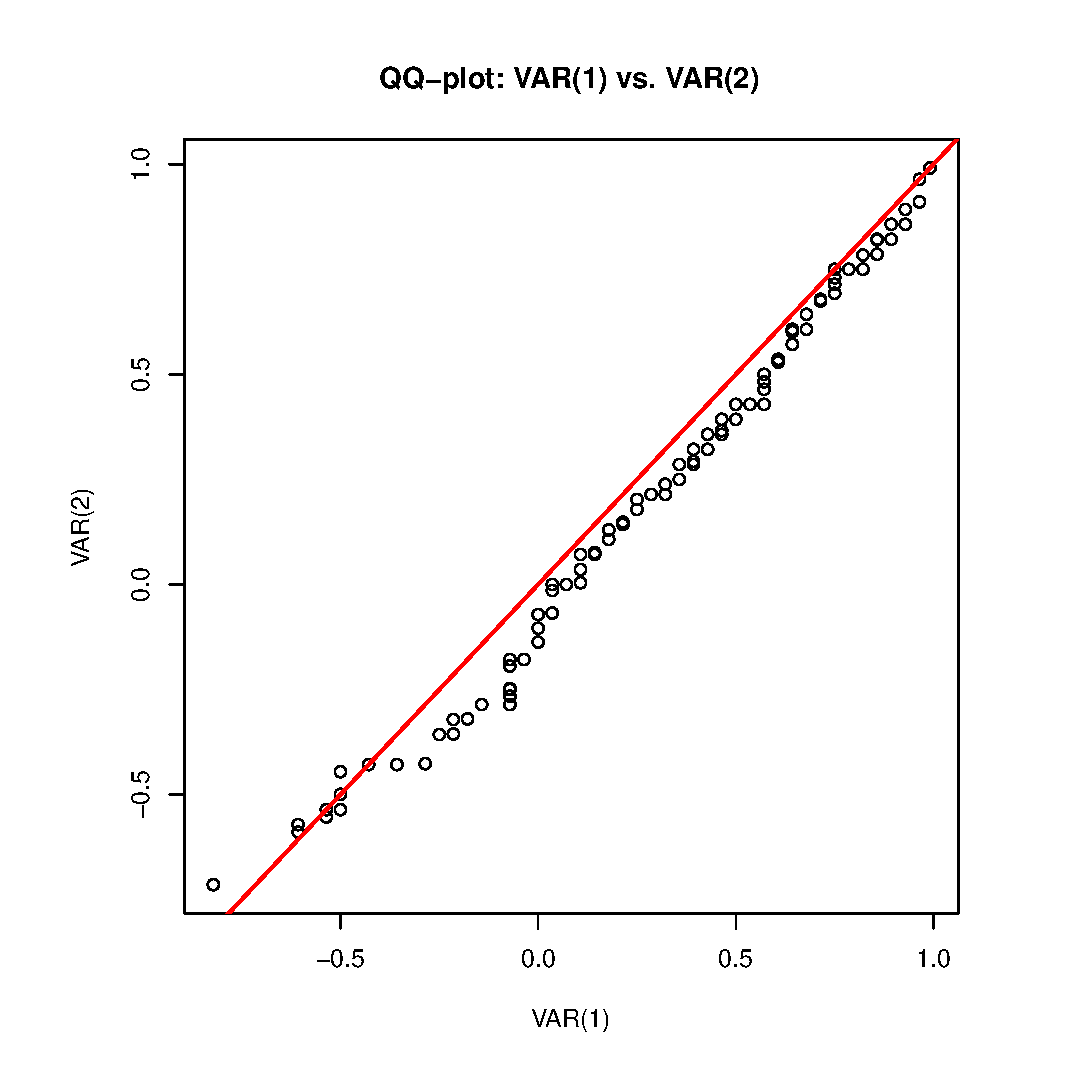
\includegraphics[scale=0.275]{Figure_7c.eps}
\end{tabular}
\caption{Histogram of Spearman correlations between the observations and VAR(1) and VAR(2) model fits (left and right penal, respectively). The third panel contains the QQ-plot of these two types of correlation.} \label{fig:compVAR1-2}  
\end{figure}


\begin{figure}[h!]
\centering
\begin{tabular}{c}
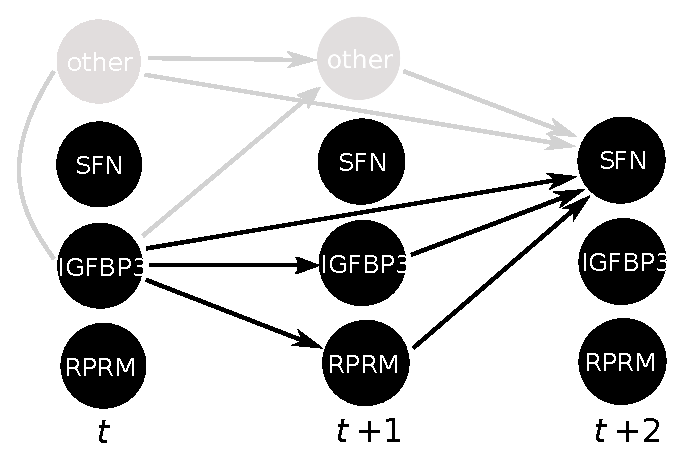
\includegraphics[scale=0.58]{VAR2pathsExample.eps}
\end{tabular}
\caption{Subgraph of the VAR(2) associated time-series chain graph, containing all paths connecting the IGFBP3 and SFN genes.}
\label{fig:VAR2pathDecomposition}  
\end{figure}


The covariance of the expression levels of a gene at the current time point and that of another gene at a future time point may be decomposed in terms of the paths connecting them in the time series chain graph, thus clarifying the propagation of signals through the network. In general, the covariance between the $j_1$- and $j_2$-th variates at time points $t$ and $t + \tau$, respectively, is:
%\begin{eqnarray*}
\begin{flalign*}
\mbox{Cov}(\mathbf{Y}_{j_1, t, i}, \mathbf{Y}_{j_2, t+\tau, i} \, | \, \mathbf{Y}_{\ast, t -1, i}, \mathbf{Y}_{\ast, t -2, i}) & = & \sum_{j'=1}^p (\mathbf{\Sigma}_{\varepsilon})_{j_1, j'} \sum_{ \substack{ \ell_0=0, \ell_m \in \{ 0, 1, 2\} \\ \sum \ell_m = \tau} } \Big( \prod_{m=0}^{\tau} \mathbf{A}_{\ell_m}^{\top} \Big)_{j', j_2}, \qquad
\end{flalign*}
%\end{eqnarray*}
where $\mathbf{A}_{0} = \mathbf{I}_{pp}$. The covariance can be further decomposed by expansion of the product of the (sparse) autoregression parameters $\mathbf{A}_1$ and $\mathbf{A}_2$ to obtain the contributions of all temporal paths connecting $j'$ and $j_2$ and, similarly, using the work of \cite{Jones2005} of the contemporaneous $(j_1, j')$-paths contributions. This is illustrated on the covariance between the IGFBP3 and SFN genes' expression levels two time points apart, equalling $-0.0142$. Figure \ref{fig:VAR2pathDecomposition} depicts the paths connecting these genes with the three paths contributing most to the covariance singled out. That is, the covariance is dominated by the temporal paths $Y_{\mbox{{\tiny IGFBP3}},t} \rightarrow Y_{\mbox{{\tiny SFN}},t+2}$, $Y_{\mbox{{\tiny IGFBP3}},t} \rightarrow Y_{\mbox{{\tiny IGFBP3}},t+1} \rightarrow Y_{\mbox{{\tiny SFN}},t+2}$, and $Y_{\mbox{{\tiny IGFBP3}},t} \rightarrow Y_{\mbox{{\tiny RPRM}},t+1} \rightarrow Y_{\mbox{{\tiny SFN}},t+2}$. Their contributions amount to $0.646$, $-0.0304$ and $-0.0211$, respectively, which accounts for 66.7\% (=38.3\% + 16.8\% + 11.6\%, respectively) of the absolute decomposed covariance contributions. The remaining 33.3\% is distributed over fourteen alternative paths involving seven other genes. Clearly, the IGFBP3 gene affects the SFN gene directly, but there is some attenuation via other routes of the network.



\section{Multiple VAR(1) models}
The sample information of the time-course experiment previously modelled by the VAR(1) model is now overlayed by group information (e.g. transfected by HPV16 or HPV18). One may then wish to highlight differences between the groups' time-series chain graphs. We focus on differential temporal relations between these graph. To this end we propose to estimate the autoregression coefficient matrices of the groups jointly employing the fused ridge estimator.

Still $n$ samples (cell lines) are followed over time and multivariately interrogated at regular intervals. Previously, the samples formed a single group i.i.d. distributed. Now the samples are divided in $G$ groups (e.g. induced by different treatments administered). The samples are indexed by $i=1, 2, \ldots, n_1, n_1 + 1 , \ldots, n_2, n+2 +1, \ldots 1+\sum_{g'=0}^{G-1} n_{g'}, \ldots, \sum_{g'=0}^{G} n_{g'}$ with $n_0 = 0$, $n_g$ the number of samples of the $g$-th group for $g=1, \ldots, G$, and $n=n_1+ n_2 + \ldots + n_g$. Within each group are modeled by a VAR(1) model:
%\begin{eqnarray*}
\begin{flalign*}
\left\{
\begin{array}{rclll}
\mathbf{Y}_{\ast, t, i} &  = & \bnu_1 + \mathbf{A}_1 \mathbf{Y}_{\ast, t-1, i} + \bvarepsilon_{\ast, t, i} & \mbox{for } i=1, \ldots, n_1 & \mbox{ and } t=1, \ldots, \mathcal{T},
\\
\mathbf{Y}_{\ast, t, i} &  = & \bnu_2 + \mathbf{A}_2 \mathbf{Y}_{\ast, t-1, i} + \bvarepsilon_{\ast, t, i} & \mbox{for } i=n_1+1, \ldots, n_2 & \mbox{ and } t=1, \ldots, \mathcal{T},
\\
\ldots &  = & \ldots & \ldots
\\
\mathbf{Y}_{\ast, t, i} &  = & \bnu_G + \mathbf{A}_G \mathbf{Y}_{\ast, t-1, i} + \bvarepsilon_{\ast, t, i} & \mbox{for } i=n_{G-1}+1, \ldots, n_G & \mbox{ and } t=1, \ldots, \mathcal{T}.
\end{array}
\right.
\end{flalign*}
%\end{eqnarray*}
where $\mathbf{Y}_{*,t,i}$ and $\bvarepsilon_{\ast,  t, i}$ $p$-dimensional random vectors representing respectively the variates and innovations. The latter with the usual normality assumption accompanying the VAR(1) model. Per group this gives three parameters $\bnu_g$, $\mathbf{A}_g$ and $\mathbf{\Sigma}_{\varepsilon, g}$. As before we assume $\bnu_g = \mathbf{0}_p$ for all $g$ (an assumption satisfied through (variate$\times$sample)-wise centering of the data). In principle, the remaining parameters could be estimated in group-wise fashion using the machinery developed by 
\cite{Miok2017}. However, groups need not differ (substantially) and much of the structure of VAR-processes is shared among the groups. For instance, different human papilloma viruses inserted in the same cell line may affect the gene-gene interactions of a pathway differently, but are unlikely to redesign the interaction patterns completely. Would such a scenario be plausible, it is then inefficient to estimate the parameters per group separately. The estimation may benefit when information among samples is borrowed. This is done in two ways. First, we assume the innovations stem from the same distribution through $\mathbf{\Sigma}_{\varepsilon, g} = \mathbf{\Sigma}_{\varepsilon}$ for all $g$.  This need not be realistic, but primary interest is in the temporal relations among variates captured by the auto-regression parameters $\mathbf{A}_1, \ldots, \mathbf{A}_G$. Practically (and of secondary importance), this assumption avoids the inclusion of (an) additional penalty parameter(s). More importantly, further information among the groups is borrowed in the estimation of the  $\mathbf{A}_g$'s. This will be done through the use of a so-called fused ridge penalty, which shrinks $\mathbf{A}_g$'s towards each other should the data give rise to it and refrains from doing so if the data contains no indication in this direction.


The model parameters $\mathbf{A}_1, \ldots, \mathbf{A}_G$ and $\mathbf{\Sigma}_{\varepsilon}$ are estimated by means of fused ridge penalized maximum likelihood. This exploits the $1^{\mbox{{\tiny st}}}$ order Markov property which, together with the distributional assumptions above, gives \\ $\mathbf{Y}_{\ast,t,i}|\mathbf{Y}_{\ast,t-1,i} \sim \mathcal{N}\left(\mathbf{A}_g \mathbf{Y}_{\ast, t-1,i},\boldsymbol{\Sigma}_{\varepsilon}\right)$ for $i \in \{1+ \sum_{g'=0}^{g-1} n_{g'}, \ldots, \sum_{g'=0}^{g} n_{g'} \}$. The joint log-likelihood function, defined as the group-wise sum of the marginal log-likelihoods, is:
\begin{eqnarray*}
\mathcal{L}(\mathbf{Y};\mathbf{A}_1, \ldots, \mathbf{A}_G, \mathbf{\Omega}_{\varepsilon}) & \propto & \sum_{g=1}^{G} \sum_{i=1+n_{g-1}}^{n_g} \sum_{t=2}^{\mathcal{T}} \big[
\log ( |\mathbf{\Omega}_{\varepsilon} |)
\\
& &   - \frac{1}{2} ( \mathbf{Y}_{\ast,t,i}  - \mathbf{A}_g \mathbf{Y}_{\ast,t-1,i} )^\top \mathbf{\Omega}_{\varepsilon} ( \mathbf{Y}_{\ast,t,i} - \mathbf{A}_g \mathbf{Y}_{\ast,t-1,i} ) \big].
\end{eqnarray*}
The log-likelihood function $\mathcal{L}$ is penalized by ridge penalties on the $\mathbf{A}_g$'s and $\mathbf{\Omega}_{\varepsilon}$:
\begin{eqnarray*}
\tfrac{1}{2} (\mathcal{T} - 1) \lambda_{\omega} \sum_{g=1}^G n_g  \| \mathbf{\Omega}_{\varepsilon} - \mathbf{\Omega}_0 \|_2^2 + \tfrac{1}{2} (\mathcal{T} - 1) \lambda_a \sum_{g=1}^G n_g  \| \mathbf{A}_g -  \mathbf{A}_0 \|_2^2
\end{eqnarray*}
in combination with fused ridge penalties on $\mathbf{A}_g$'s:
\begin{eqnarray*}
&  &  \tfrac{1}{2} (\mathcal{T} - 1) \lambda_f \sum_{g_1=1}^G n_{g_1}   \sum_{ \substack{ g_2=1 \\ g_2 \not= g_1} }^G  \| \mathbf{A}_{g_1} - \mathbf{A}_{g_2} \|_2^2,
\end{eqnarray*}
where $\mathbf{A}_0$ and $\mathbf{\Omega}_0$ are non-random  target matrices common to all groups, ridge penalty parameter $\lambda_a$ and $\lambda_{\omega}$, and the fusion penalty parameter $\lambda_f$ determining the degree to which the $\mathbf{A}_g$ are shrunken towards each other.

The maximization of this fused ridge penalized log-likelihood proceeds along the same lines as that of the ridge penalized log-likelihood of the VAR(1) model. First, the estimator of each $\mathbf{A}_g$, given the others and $\mathbf{\Omega}_{\varepsilon}$, is derived. This is followed by that of $\mathbf{\Omega}_{\varepsilon}$ given those of the $\mathbf{A}_g$'s. These are combined in an iterative procedure to produce the final estimates. 

The estimators of the $\mathbf{A}_g$ are found by equating the first order derivative (w.r.t $\mathbf{A}_g$) of the fused ridge penalized log-likelihood to zero and solving for $\mathbf{A}_g$, treating the other variables as non-random. Matrix algebra similar to that used in the derivation of the ridge penalized ML estimators of the VAR(1) model parameters gives:
\begin{eqnarray*}
\mbox{vec}[ \hat{\mathbf{A}}_g(\lambda,\lambda_f) ] & = & \{ n_g (\mathcal{T}-1) [ \lambda_a + (G-1)\lambda_f ] \mathbf{I}_{p^2\times p^2} + \widehat{\mathbf{\Gamma}}_g(0) \otimes \mathbf{\Omega}_{\varepsilon} \}^{-1}
\\
& & \{ n_g (\mathcal{T}-1) [\lambda_a \mbox{vec}(\mathbf{A}_0) + \lambda_f \sum_{ \substack{ g'=1 \\ g' \not= g} }^G \mbox{vec}(\mathbf{A}_{g'}) ] + \textrm{vec} [ \mathbf{\Omega}_{\varepsilon} \widehat{\mathbf{\Gamma}}_g(-1) ] \},
\end{eqnarray*}
where $\widehat{\mathbf{\Gamma}}_g(0) = \tfrac{1}{n_g(\mathcal{T}-1)} \sum_{i=1}^{n_g}\sum_{t=2}^{\mathcal{T}} \mathbf{Y}_{\ast,t-1,i}\mathbf{Y}_{\ast,t-1,i}^{\top}$ and \\
 $\widehat{\mathbf{\Gamma}}_g(-1) = \tfrac{1}{n_g(\mathcal{T}-1)} \sum_{i=1}^{n_g} \sum_{t=2}^{\mathcal{T}} \mathbf{Y}_{\ast, t, i} \mathbf{Y}_{\ast,t-1,i}^{\top}$, the estimates of the variance and lag $-1$ covariance of the $g$-th group. For the ridge ML estimator of the common precision matrix of the innovations $\boldsymbol{\Omega}_{\varepsilon}$, we need the sample covariance matrix of the innovations:
\begin{eqnarray*}
\mathbf{S}_{\varepsilon} =
\sum_{g=1}^{G} \frac{1}{n_g(\mathcal{T}-1)}
\sum_{i=1+n_{g-1}}^{n_g} \sum_{t=2}^{\mathcal{T}} \left[\mathbf{Y}_{\ast,t,i} - \mathbf{A}_g \mathbf{Y}_{\ast,t-1,i} \right] \left[\mathbf{Y}_{\ast,t,i} - \mathbf{A}_g\mathbf{Y}_{\ast,t-1,i} \right]^{\top}.
\end{eqnarray*}
The ridge estimate of $\boldsymbol{\Omega}_{\varepsilon}$ is then (with the same properties) as in the VAR(1) case only with this sample covariance matrix replacing that of the non-fused case.

The estimators above are combined in an iterative procedure to obtain the joint ML estimators of the $\mathbf{A}_g$'s and $\boldsymbol{\Omega}_{\varepsilon}$. The procedure is initiated with the marginal ridge LS estimates of the $\mathbf{A}_g$'s. These are obtained through the group-wise fit of  the VAR(1) model with $\boldsymbol{\Omega}_{\varepsilon} = \mathbf{I}_{pp}$. The first step of the iterative estimation procedure then comprises the estimation of $\boldsymbol{\Omega}_{\varepsilon}$ (given the initial estimates of $\mathbf{A}_g$). This is followed by the estimation of the $\mathbf{A}_g$'s. Running over the groups, each $\mathbf{A}_g$ is estimated keeping the other $\mathbf{A}_g$'s and $\boldsymbol{\Omega}_{\varepsilon}$ fixed. This is done until sequential estimates of each $\mathbf{A}_g$ differ less than a user-specified threshold. Once this is achieved, the procedure returns to the estimation of $\boldsymbol{\Omega}_{\varepsilon}$. And so on, until convergence.


The methodology for joint learning of multiple VAR(1) models through the fused ridge approach is illustrated on mRNA gene expression data from the aforementioned experiment with HPV16 and HPV18 group information overlayed. The optimal penalty parameters selected through maximization of the LOOCV log-likelihood are $\lambda_a=19.4444$, $\lambda_f=21.9996$ and $\lambda_{\omega}=0.0024$. Their optimality has been be checked visually by contour plots of the LOOCV log-likelihood versus penalty parameters (Figure 4.3, \cite{Supp2018}). Using the optimal penalty parameters non-sparse model parameters $\mathbf{A}_g$ and $\boldsymbol{\Omega}_{\varepsilon}$ are estimated.


The support of the model parameters is determined from the fused ridge parameter estimates. Sparsification of the $\mathbf{A}_g$'s and $\boldsymbol{\Omega}_{\varepsilon}$ proceeds as for VAR(1) model (cf. \cite{Miok2017}) with the support being determined for each of the $g$ autoregressive model parameter separately. The inferred number of nonzero autoregression parameters is 88 and 125 for the HPV16 and HVP18 affected cell lines, respectively. The excess of inferred interactions of the HPV18 cell line model may be due to the HPV16 being more oncogenic than the HPV18. The HPV16 may achieve this through more aggressive disruption of the cellular regulatory network, leading to less preserved interactions. Fewer interactions indicate less cohesion, in turn corresponding to less control of the network and increasing the potential for oncogenesis \citep{Wieringen2015}. This observation might be linked to the varying degree in p53 degradation observed for different oncogenic HPV types \citep{Schutze2014}. Inferred (non)-zero elements of the $\mathbf{A}_g$'s and $\boldsymbol{\Omega}_{\varepsilon}$ are then used to re-estimate these parameters, but per group the VAR(1) model is now fitted separately due to their support being different. The group-wise optimal penalty parameters are $\lambda_{a}=1.4077$, $\lambda_{\omega}=0.0045$ for cell lines affected with HPV16 and $\lambda_{a}=1.0967$, $\lambda_{\omega}= 0.0053$ for those affected with HPV18. The optimality of the penalty parameters are verified using contour plots. The penalty parameters $\mathbf{A}$ and $\mathbf{\Omega}_{\varepsilon}$ are comparable in size between the groups. The resulting group-wise re-estimated -- incorporating the inferred support -- model parameters are thus also comparable. The overlap and contrast of the HPV16 and HPV18 time-series chain graph derived from the re-estimated VAR(1) parameters for both groups are displayed in Figure \ref{fig:VARmultipleEst}. This reveals a substantial amount of overlap but even more differences, with plenty of virus specific edges. 

\begin{figure}[h!]
\centering
\begin{tabular}{cccc}
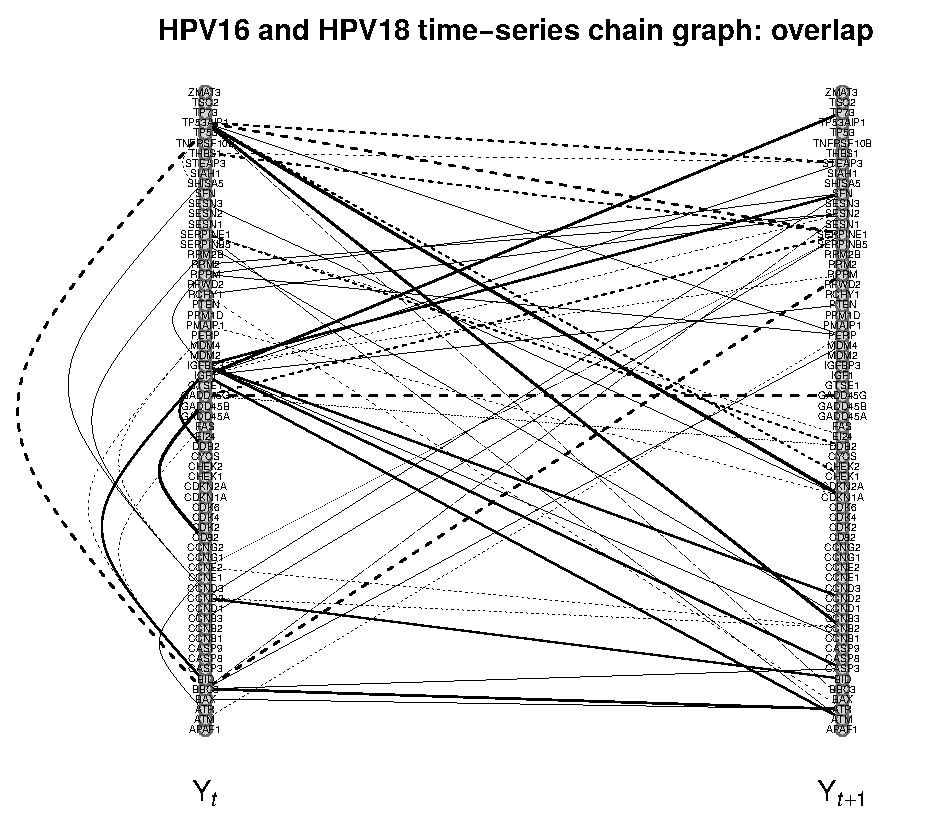
\includegraphics[scale=0.47]{Figure_11c.eps} & & &
\includegraphics[scale=0.45]{Figure_11d.eps}
\end{tabular}
\caption{Left and right panels depict the overlap and contrast, respectively, of the inferred time-series chain graphs from the cell lines affected with HPV16 and HPV18. Solid and dashed lines represent positive and negative relations, respectively. Black lines are common to the time-series chain graphs of both viruses, while the  blue and red lines are present in the graphs of the HPV16 and HPV18 (respectively) only. The thickness of the lines corresponds to the strength of the relation.}
\label{fig:VARmultipleEst}
\end{figure}


Post-estimation analysis of the VAR(1) model may shed light on the differential gene expression dynamics implied by different VAR(1) models. This is done by the downstream analyses introduced for the VAR(1) model. For instance, group-wise impulse response analysis may reveal how  a unit change in gene expression levels at the current time point $t$ differentially affects the gene expression level at time point $t+\tau$. Similarly, the differentially association between a variate at the current time and those at a future time may be identified from the group-wise mutual informations. Finally, comparison of group-wise path decompositions may point to the cross-group re-wiring of the connectivity of two nodes. Downstream analysis using re-estimated model parameters may also comprise of the calculation of network summary measures \citep{Newman2010}. For the five top `regulators' and `regulatees' node statistics are calculated and shown in Table \ref{table:postEstNodeStats} for the HPV16 and HPV18  cell lines. Comparison of both table reveals that there is a large overlap in `regulators' and `regulatees'. In both gene-type categories there is a notable difference. IGF1 and CCNB3 are a top `regulator' and `regulatee', respectively, in the VAR(1) description of the P53 signalling pathway from the HPV16. These are replaced by CCND2 and PERP, respectively, in the HPV18 data based pathway model. These differences shed light on the differential oncogenic potential of the two HPV varieties as was also shown by differences in immortalising capacity related to copy number alterations {\cite{Schutze2014, Schutze2016}.


\begin{table}
\caption{Node statistics for the top five `regulators' and `regulatees' (as derived from the time-series chain graph of the p53 signaling pathway) identified from the HPV16 and HPV18 affected cell line data using the estimated VAR(1) models. The left most column indicates the HPV variant, followed by the names of these genes. The next columns give the following node statistics: the in- and out-degree of the lag-one temporal dependencies; betweenness in the (global) partial correlation graph, closeness in the (global) partial correlation graph, the mutual information between the expression level of the gene at time $t$ and all other genes from the pathway at time $t+1$, and the impulse response in the gene at time $t$ on all other genes at time $t+1$.}
\begin{tabular}{ll*{6}{c}r}
\hline
\hline          
HPV & gene & $\mbox{deg}^-(\mathbf{A})$ & $\mbox{deg}^+(\mathbf{A})$ & betw. & close. & mut. info. & imp. resp.  \\
\hline
16 & BBC3        & 0 & 12 & 27 & 0.00029 & 0.08711 & 0.01584
\\
16 & IGF1     & 0 & 11 & 0 & 0.00025 & 0.03266 & 0.01112
\\
16 & IGFBP3     & 0 & 10 & 17 & 0.00029 & 0.09925 & 0.01798
\\
16 & TP53AIP1     & 1 & 9 & 1 & 0.00025 & 0.11136 & 0.01536
\\
16 & THBS1     & 0 & 6 & 0 & 0.00024 & 0.03132 & 0.00882
\\
\\
16 & CCNB3    & 10 & 1 & 0 & 0.00024 & 0.00065 & 0.00042
\\
16 & SESN2        & 7 & 1 & 0 & 0.00024 & 0.02017 & 0.00176
\\
16 & SERPINE1       & 6 & 5 & 0 & 0.00024 & 0.04194 & 0.00683
\\
16 & STEAP3    & 5 & 0 & 0 & 0.00024 & 0.00000 & 0.00000
\\
16 & CDKN2A  & 5 & 0 & 0 & 0.00024 & 0.00000 & 0.00000
\\
\\
\\
18 & IGFBP3        & 0 & 17 & 17 & 0.0029 & 0.16543 & 0.02502
\\
18 & CCND2     & 1 & 15 & 24 & 0.0029 & 0.02642 & 0.01705
\\
18 & BBC3     & 0 & 15 & 27 & 0.0029 & 0.09903 & 0.02233
\\
18 & TP53AIP1     & 0 & 10 & 1 & 0.0028 & 0.05642 & 0.01784
\\
18 & THBS1     & 1 & 11 & 0 & 0.0028 & 0.09053 & 0.01906
\\
\\
18 & PERP    & 12 & 0 & 0 & 0.0027 & 0.00000 & 0.00000
\\
18 & SERPINE1        & 7 & 3 & 0 & 0.0027 & 0.02247 & 0.00465
\\
18 & CDKN1A       & 6 & 0 & 0 & 0.0025 & 0.00000 & 0.00000
\\
18 & STEAP3 & 5 & 0 & 0 & 0.0025 & 0.00000 & 0.00000
\\
18 & SESN2  & 5 & 1 & 0 & 0.0026 & 0.00016 & 0.00023
\\
\hline
\hline
\end{tabular}
\label{table:postEstNodeStats}
\end{table}


Finally, the path decomposition analysis of the covariance -- outlined for the VAR(1) model -- is applied to the HPV16 and HPV18 VAR(1) models seperately to identify differential regulatory patterns. This is done for the (IGFBP3, SESN2) gene pair and we thus decompose $\mbox{Cov}(Y_{IGFBP3,t}, Y_{SESN2,t+1}) = (\mathbf{\Sigma}_{\varepsilon} \mathbf{A}^{\top})_{IGFBP3,SESN2}$. Although this reveals quantitative differences between the two decompositions, the details are omitted. More strikingly, the direct path between $Y_{IGFBP3,t}\rightarrow Y_{SESN2,t+1}$ has vanished in the HPV18 description of the P53 pathway. This hints at differential regulation.

\section{The VARX(1) model} 
When having measured multiple molecular levels, an integrative view of the levels' networks  comes within reach. In addition to the `within-level' relations among variates, this also encompasses relations between different molecular levels (e.g. how does a DNA copy number change affect a gene's mRNA expression levels). Here this is done by extending the VAR(1) model to a VARX(1) model which allows the inclusion of time-varying covariates (responsible for the X in VARX) like DNA copy number or microRNA expression. Within the VARX(1) model the molecular levels are no longer on a par. It differentiates between an endogeneous (e.g. mRNA expression) and an exogeneous level (e.g. DNA copy number). In addition to the `between-level' relations that may now be reconstructed, the inclusion of the exogeneous level aids in the reconstruction of the underlying network of the endogeneous one. 

Consider a time-course microarray experiment comprising $n$ cell lines (samples) that followed during $\mathcal{T}$ consecutive time points. At each time point, all samples' variates stemming from multiple molecular levels (at least two e.g. DNA copy number, mRNA or miRNA gene expression) are measured. The endogeneous variates (e.g. the mRNA gene expression levels) of sample $i$ at time point $t$ are represented by the $p$-dimensional random vector $\mathbf{Y}_{*,t,i}$. Similarly, the $q$-dimensional variable $\mathbf{X}_{*,t,i}$ denotes the exogeneous variates (e.g. DNA copy number or miRNA gene expression levels) of sample $i$ at time point $t$.


Let the data from this experiment be modeled by a first-order vector autoregressive with a time-varying covariate, abbreviated to VARX(1), model:
\begin{eqnarray*}
\mathbf{Y}_{*,t,i} & = & \boldsymbol{\nu}+\mathbf{A} \mathbf{Y}_{*,t-1,i} + \mathbf{B} \mathbf{X}_{*,t,i} + \boldsymbol{\varepsilon}_{*,t,i},
\end{eqnarray*}
with intercept vector $\nu=\mathbf{0}_{p}$, $q$-dimensional exogenous time-varying covariate vector $\mathbf{X}_{*,t,i}$ of sample $i$ at time $t$, the $p \times p$-dimensional matrix $\mathbf{A}$ with auto-regression coefficients, the $p \times q$-dimensional matrix $\mathbf{B}$ with regression coefficients of the time-varying covariates, and $\boldsymbol{\varepsilon}_{*,t,i}$ an error vector of length $p$. The errors are assumed to be identically and independently distributed as $\boldsymbol{\varepsilon}_{*,t,i} \sim \mathcal{N}( \mathbf{0}, \mathbf{\Sigma}_{\varepsilon})$.

Due to the independence among the samples and the Markov property of the VARX(1) model, the likelihood is:
\begin{eqnarray*}
\hspace{-1.0cm} L(\mathbf{Y};\mathbf{X},\mathbf{A},\mathbf{B},\boldsymbol{\Sigma}_{\varepsilon}) & = & \prod_{i=1}^n \prod_{t=2}^{\mathcal{T}}P(\mathbf{Y}_{*,t,i}|\mathbf{Y}_{*,t-1,i},\mathbf{X}_{*,t,i}).
\end{eqnarray*}
Use $\mathbf{Y}_{*,t,i} \, | \, \mathbf{Y}_{*,t-1,i},\mathbf{X}_{*,t,i}\sim \mathcal{N}\left(\mathbf{A} \mathbf{Y}_{*,t-1,i} + \mathbf{B} \mathbf{X}_{*,t,i},\boldsymbol{\Sigma}_{\varepsilon}\right)$ and take the logarithm to obtain the log-likelihood:
%\begin{eqnarray*}
\begin{flalign*}
\mathcal{L}(\mathbf{Y};\mathbf{X}, \mathbf{C}, \boldsymbol{\Sigma}_{\varepsilon}) & \propto &  - n(\mathcal{T}-1)\ln\left|\boldsymbol{\Sigma}_{\varepsilon}^{-1}\right|  -\frac{1}{2}\sum_{i=1}^n \sum_{t=2}^{\mathcal{T}}\left\{-\frac{1}{2}\left[\mathbf{Y}_{*,t,i}-  ( \mathbf{Z}_{*,t,i}^\top \otimes \mathbf{I}_{p\times p} ) \textrm{vec}(\mathbf{C}) \right]^\top\right. \qquad \qquad \qquad \qquad \qquad 
\\
& & \left.\boldsymbol{\Sigma}_{\varepsilon}^{-1}
\left[\mathbf{Y}_{*,t,i}-  (\mathbf{Z}_{*,t,i}^\top \otimes \mathbf{I}_{pp} ) \textrm{vec}(\mathbf{C}) \right] \right\}, \qquad \qquad \qquad \qquad  \qquad \qquad
%\end{eqnarray*}
\end{flalign*}
in which $\mathbf{C} = (\mathbf{A}|\mathbf{B})$ and thus $\textrm{vec}(\mathbf{C}) = \textrm{vec}(\mathbf{A}|\mathbf{B}) = [\textrm{vec}(\mathbf{A})^{\top},  \textrm{vec}(\mathbf{B})^\top ]^{\top}$, where the vec-operator stacks the columns of matrix into a vector. Moreover, $\mathbf{Z}_{*,t,i} = (\mathbf{Y}_{*,t-1,i}^{\top},  \mathbf{X}_{*,t,i}^{\top})^{\top}$.

To accommodate the high-dimensionality of the data the log-likelihood
is augmented with ridge penalties on $\mathbf{A}$, $\mathbf{B}$ and $\mathbf{\Sigma_{\varepsilon}}$:
\begin{eqnarray*}
& & \hspace{-2cm} \mathcal{L}^{\mbox{{\tiny pen}}}(\mathbf{Y};\mathbf{X},\mathbf{C},\boldsymbol{\Omega}_{\varepsilon};\lambda_a,\lambda_b,\lambda_{\omega},\mathbf{C}_0, \boldsymbol{\Omega}_0)
\\
& \propto & \mathcal{L}(\mathbf{Y};\mathbf{X},\mathbf{C}, \boldsymbol{\Omega}_{\varepsilon}) -\frac{n(\mathcal{T}-1)}{2}\lambda_{\omega}\textrm{tr}\left[(\boldsymbol{\Omega}_{\varepsilon}-\boldsymbol{\Omega}_{0})^\top(\boldsymbol{\Omega}_{\varepsilon}-\boldsymbol{\Omega}_{0})\right]
\\
& & -\frac{n(\mathcal{T}-1)}{2}\textrm{tr}\left\{\left[\textrm{vec}( \mathbf{C})-\textrm{vec}(\mathbf{C}_0) \right]^\top \mathbf{\Lambda}_c \left[\textrm{vec} (\mathbf{C})-\textrm{vec}(\mathbf{C}_0) \right]\right\}
\end{eqnarray*}
in which $\boldsymbol{\Omega}_{\varepsilon} = \boldsymbol{\Sigma}_{\varepsilon}^{-1}$, user-specified, non-random target matrices $\mathbf{A}_0$, $\mathbf{B}_0$ and $\mathbf{\Omega}_0$, $\mathbf{C}_0 = (\mathbf{A}_0 | \mathbf{B}_0)$, and the $p(p+q) \times p(p+q)$ dimensional, diagonal matrix $\mathbf{\Lambda}_c$ with $(\mathbf{\Lambda}_c)_{jj} = \lambda_a$ for $j = 1, \ldots, p^2$ and $(\mathbf{\Lambda}_c)_{jj} = \lambda_b$ for $j = p^2 + 1, \ldots, p^2 + pq$. Note that this penalty term involving $\mathbf{C}$ is proportional to the algebraic ridge penalties $\| \mathbf{A} \|^2_2 + \| \mathbf{B} \|^2_2$.

An estimator for  $\mathbf{C}$ is now found by solving its estimating equation (arrived at through equating the derivative of the penalized log-likelihood with respect to $\mathbf{C}$ to zero). Grouping of terms and solving for $\mathbf{C}$ yields the ridge ML estimator:
\begin{eqnarray*}
\textrm{vec} [\widehat{\mathbf{C}}(\boldsymbol{\Lambda}_c) ] & = & [\boldsymbol{\Lambda}_c+\tilde{\boldsymbol{\Gamma}}_{zz}(0) \otimes \boldsymbol{\Omega}_{\varepsilon} ]^{-1} \{\boldsymbol{\Lambda}_c\textrm{vec}(\mathbf{C}_0) + \textrm{vec}  [\boldsymbol{\Omega}_{\varepsilon} \otimes \tilde{\boldsymbol{\Gamma}}_{yz}(-1) ] \},
\end{eqnarray*}
where
%\begin{eqnarray*}
\begin{flalign*}
\tilde{{\boldsymbol{\Gamma}}}_{zz}(0)=\frac{1}{n(\mathcal{T}-1)}\sum_{i=1}^{n}\sum_{t=2}^{\mathcal{T}} \mathbf{Z}_{*,t,i}\mathbf{Z}_{*,t,i}^{\top} \quad \mbox{ and  } \quad \tilde{\boldsymbol{\Gamma}}_{yz}(-1) = \frac{1}{n(\mathcal{T}-1)} \sum_{i=1}^{n} \sum_{t=2}^{\mathcal{T}}\mathbf{Y}_{*,t,i} \mathbf{Z}_{*,t,i}^{\top}.
\end{flalign*}
%\end{eqnarray*}
The ridge estimator of $\mathbf{C}$ involves the Kronecker product which frustrates its numerical evaluation for even moderately sized $p$ and $q$ (as it involves matrices of dimensions $(p^2 + pq) \times (p^2 + pq)$. Previously with the VAR(1) model, this was circumvented by rewriting the estimator. The same can be done here, but requires an approximation of the inverse in the ridge estimator of $\mathbf{C}$. For the approximation, write $\nu_1 = {\textstyle\frac{1}{2}} (\lambda_a + \lambda_{b})$ and $\nu_2 = {\textstyle\frac{1}{2}} (\lambda_a - \lambda_{b})$. Then:
\begin{flalign*}
%\begin{eqnarray*}
[\boldsymbol{\Lambda}_c + \tilde{\boldsymbol{\Gamma}}_{ZZ}(0) \otimes \boldsymbol{\Omega}_{\varepsilon}]^{-1} & = & \left[ \nu_1 \mathbf{I}_{p(p+q) \times p(p+q)} + \nu_2
\left(
\begin{array}{rr}
\mathbf{I}_{p^2 \times p^2} & \mathbf{0}_{p^2 \times pq}
\\
\mathbf{0}_{pq \times p^2} & - \mathbf{I}_{pq \times pq}
\end{array}
\right)
+ \tilde{\boldsymbol{\Gamma}}_{ZZ}(0) \otimes \boldsymbol{\Omega}_{\varepsilon} \right]^{-1} 
\\
& \approx & \mathbf{\Theta}^{-1} - \nu_2 \mathbf{\Theta}^{-1} \left(
\begin{array}{cc} \mathbf{I}_{p^2 \times p^2} & \mathbf{0}_{p^2 \times pq}
\\
\mathbf{0}_{pq \times p^2} & - \mathbf{I}_{pq \times pq}
\end{array}
\right) \mathbf{\Theta}^{-1} \qquad \qquad \qquad \qquad \quad
\\
& = & \mathbf{\Theta}^{-1} - \nu_2 \mathbf{\Theta}^{-2}  + 2 \nu_2 \mathbf{\Theta}^{-1} \left(
\begin{array}{cc} \mathbf{0}_{p^2 \times p^2} & \mathbf{0}_{p^2 \times pq}
\\
\mathbf{0}_{pq \times p^2} & - \mathbf{I}_{pq \times pq}
\end{array} \right) \mathbf{\Theta}^{-1}, \qquad \qquad
%\end{eqnarray*}
\end{flalign*}

where $\mathbf{\Theta} =  \nu_1 \mathbf{I}_{p(p+q) \times p(p+q)}
+ \widetilde{\boldsymbol{\Gamma}}_{ZZ}(0)\otimes\boldsymbol{\Omega}_{\varepsilon}$.
The eigen-decomposition can readily be applied to the first two terms in the approximation. But also to the last as only a subset of the eigenvectors share the same nonzero eigenvalue.

Again the ridge ML estimator of the error precision, $\boldsymbol{\Omega}_{\varepsilon}$, is given in display (\ref{ridgePrecision}) with the sample error covariance now:
%\begin{eqnarray*}
\begin{flalign*}
\mathbf{S}_{\varepsilon} = \frac{1}{n(\mathcal{T}-1)}\sum_{i=1}^{n}\sum_{t=2}^{\mathcal{T}}\left[\mathbf{Y}_{*,i,t}- \mathbf{A}\mathbf{Y}_{*,t-1,i} - \mathbf{B} \mathbf{X}_{*,t,i} \right] \left[\mathbf{Y}_{*,t,i} - \mathbf{A} \mathbf{Y}_{*,t-1,i} - \mathbf{B} \mathbf{X}_{*,t,i}\right]^{\top},
\end{flalign*}
%\end{eqnarray*}
substituted. 

The ridge penalized maximum likelihood estimates of $\mathbf{A}$, $\mathbf{B}$ and $\boldsymbol{\Omega}_{\varepsilon}$ may now be obtained by iteratively estimating one while keeping the other fixed. This iterative procedure is initiated by the ridge LS (least squares) estimate of $\mathbf{C}$, which is obtained from its ML counterpart by setting $\boldsymbol{\Omega}_{\varepsilon} = \mathbf{I}_{pp}$. As before penalty parameters $\lambda_a$, $\lambda_b$ and $\lambda_{\omega}$ are chosen to optimize the LOOCV log-likelihood.

Next we present the several downstream analyses in order to gain better understanding of the dynamics within and between the entities of the various molecular levels. 
\begin{compactitem}
\item  First the nonzero elements of model parameters $\mathbf{A}$, $\mathbf{B}$ and $\boldsymbol{\Omega}_{\varepsilon}$ are identified through sparsification (in a similar way as for the VAR(1) model). 

\item The impulse response analysis of the VARX(1) model assesses the effect of a change in an innovations or a time-varying covariate on a particular variate. This amounts to the evaluation of the derivative of the latter with respect to one of the former. Using the time-recursive definition of the VARX(1) model, this boils down to:
\begin{eqnarray*}
\frac{\partial \mathbf{Y}_{\ast,t+\tau,i}}{\partial \boldsymbol{\varepsilon}_{\ast,t,i}} & = & \mathbf{A}^{\tau} \qquad \mbox{ and } \qquad \frac{\partial \mathbf{Y}_{\ast,t+\tau,i}}{\partial \mathbf{X}_{\ast,t,i}} \, \, \,  = \, \, \,  \mathbf{A}^{\tau} \mathbf{B},
\end{eqnarray*}
with $\tau \in \mathbb{N}$. The $(j,k)$-th element of $\mathbf{A}^{\tau}\mathbf{B}$ represents the change in $Y_{j,t+\tau, i}$ due a unit change in $X_{k,t,i}$.

\item In the explanation of $\mathbf{Y}_{\ast, t, i}$ the VARX(1) model assumes the time-varying covariates to be non-random. When evaluating the mutual information terms involving any of the $\mathbf{X}_{j, t, i}$'s drop out. As a result conditional variances involved in the mutual information equal to that of the VAR(1) model, for which we refer to \cite{Miok2017}.
\end{compactitem}

The VARX(1) model related methodology is applied on the P53 signalling pathway data from the HPV-induced cell line experiment. In this interactions between the genes' DNA copy number and microRNAs on one hand and the mRNAs on the other are assumed to be known. With respect to the former only \textit{cis}-interactions are assumed to be physically feasible: a gene's dosage may only affect its own transcription directly (which in turn may then indirectly propagate through the network). The microRNA-mRNA interactions are taken from microRNA target prediction data bases. In particular, a microRNA-mRNA interaction requires for the mRNA to be the microRNA's target in at least two out of three data bases (targetscan, mirDB and RNA22). Optimal penalty parameters ($\lambda_a=255$, $\lambda_b=130$ and $\lambda_{\omega}=0.0034$) are verified using contour plots (Figure 4.3, \cite{Supp2018}) and used to arrive at estimates of the VARX(1) model parameters $\mathbf{A}$, $\mathbf{B}$ and $\mathbf{\Omega}_{\varepsilon}$. Support of the model parameters $\mathbf{A}$ and $\mathbf{\Omega}_{\varepsilon}$ is determined using the post-estimation selection procedure described earlier. 

The support of model parameters $\mathbf{A}$ and $\boldsymbol{\Omega}_{\varepsilon}$ (that of $\mathbf{B}$ is assumed known) is inferred through sparsification of their ridge estimates. The inferred support is used to re-estimate the model. Optimal penalty parameters are re-determined ($\lambda_a=0.6$, $\lambda_b=0.4868$ and $\lambda_{\omega}=0.0001$) and verified through contourplots (not shown). In Figure 4.4, \cite{Supp2018} the re-estimated model parameters are visualized as heatmaps, here only the time-series chain graph induced by these parameter is shown (Figure \ref{fig:graphVARX1})

\begin{figure}[h!]
\centering
\begin{tabular}{cc}
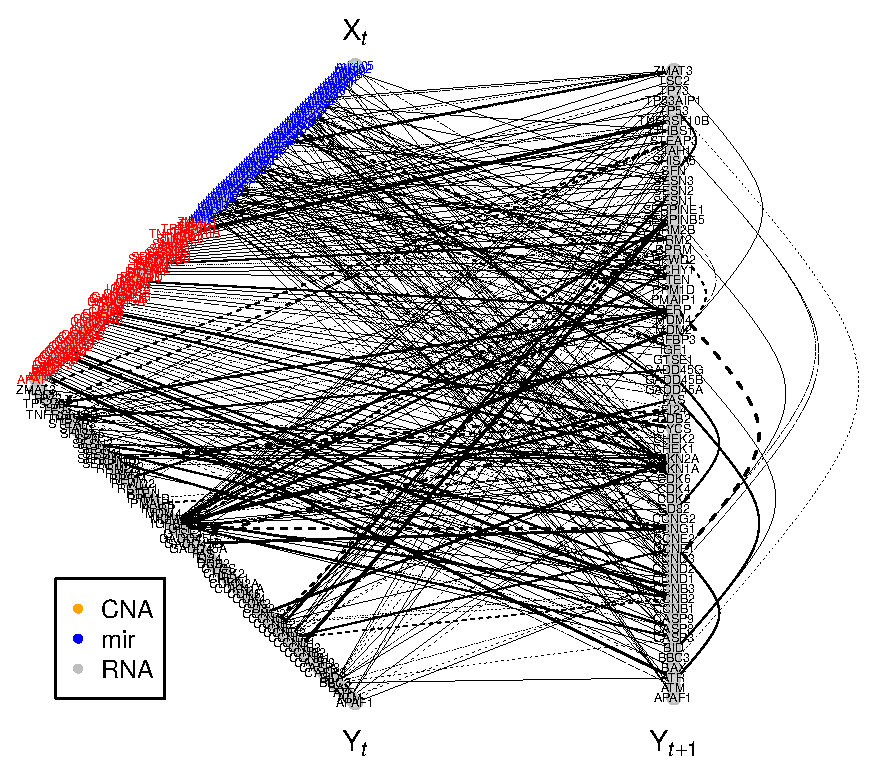
\includegraphics[scale=0.6]{Figure_17.eps}
\end{tabular}
\caption{Inferred time-series chain graph corresponding to the estimated VARX(1) model. Solid and dashed lines represent positive and negative relations, respectively. Line thickness corresponds to the strength of the relation. Unconnected nodes have been pruned from the graph.}
\label{fig:graphVARX1}
\end{figure}

The model parameters -- re-estimated obeying the inferred support -- are studied. We first turn our attention to the estimated matrix $\mathbf{B}$. The coefficients related to the DNA copy number effect are overwhemingly positive (as can be witnessed from the parameter heatmaps provided in Figure 4.4, \cite{Supp2018} or from the solid edges originating from the DNA copy number related nodes in Figure \ref{fig:graphVARX1}). This confirms the common-sense `larger gene dosage, more transcription' hypothesis. For miRNAs, (among others) breaking down mRNAs post-transcriptionnally, negative estimates of their effects are expected. Indeed, the largest (in an absolute sense) estimates are negative, but generally the miRNA related coefficients are a mixed bag containing both positive and negative estimates. As multiple miRNAs are known to target the same mRNA and proteins encoded by these mRNAs on the other hand could be involved in transcriptional regulation of the miRNAs, it is likely that many indirect effects are detected on the RNA level as well.


\begin{figure}[h!]
\centering
\begin{tabular}{c}
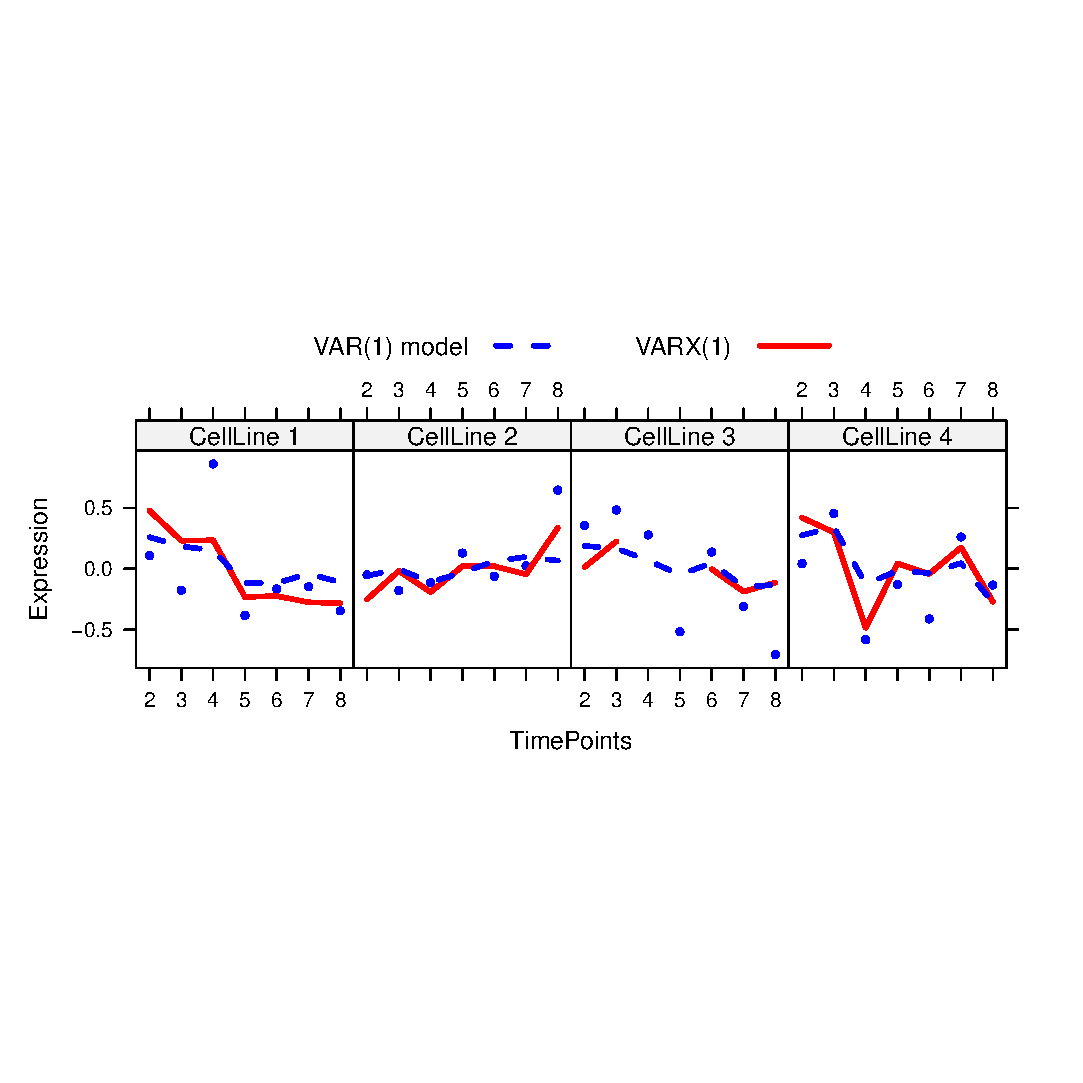
\includegraphics[scale=0.8]{Figure_14.eps}\\
\end{tabular}
\caption{Observations and VAR(1) and VARX(1) model fits of the CCNG1 expression data. Each panel, one per cell line, plots gene expression against time, excluding the first time point. The solid red and dashed green curves represents the fit of the VARX(1) and VAR(1) model fits, respectively. In the third cell line the VARX(1) model fit is interrupted due to failed microRNA hybridizations. 
}
\label{fig:CCNG1fitVAR1-VARX1}  
\end{figure}


The fitted VAR(1) and VARX(1) models exhibit various differences. Comparison of the temporal relations contained in the matrix $\mathbf{A}$ reveals only small changes in the endogenous part of the VAR(1) and VARX(1) models. For instance, both models share the same top `regulators', although these `regulators' affect more genes in VARX(1) model. Alternatively, both models may be compared by the study of their fit. Figure \ref{fig:CCNG1fitVAR1-VARX1} shows both fits for the gene CCNG1. More globally, the cell line-wise Spearman correlations between fitted and observed values of each gene may be compared between both models. Figure 4.8, \cite{Supp2018} contains the histograms of these correlations for VAR(1) and VARX(1) models. Notice that VARX(1) model has more correlations on right-hand side -- the positive part of the $x$-axis -- which implies an overall better fit. This improvement in fit is due a more complex model, using exogenous variables (DNA copy number and miRNA gene expression). To put this in perspective, the matrix $\mathbf{A}$ of the VAR(1) model contains 134 non-zero parameters, while the matrices $\mathbf{A}$ and $\mathbf{B}$ of VARX(1) model have 126 and 235 non-trivial parameters, respectively. 



\section{Conclusion}
The paper discussed the learning of molecular network models from high-dimensional multilevel molecular time-course data. This comprised their estimation, through penalized parameter estimation and support reconstruction,  as well as their exploitation to produce tangible consequences for the medical collaborator. Throughout the \texttt{ragt2ridges}-package, implementing the presented methodology, was used as a powerful means to this end. In the application of the developed methodology to a cervical study, serving as a running example, its potential for versatile analyses of the high-dimensional time-series omics data was demonstrated.

Further methodological and software development is envisioned in two directions. The most pressing is to facilitate analyses presented here using next generation sequencing data. As these data represent actual counts rather than intensities believed to be proportional to these counts, the Gaussian assumption of the presented models is untenable and need to be replaced by a more suitable alternative for sequencing data \citep{Heinen2003}. On the hand, all presented analyses assume linear relationships among the molecular entities. As a simple first order approximation this may be fine, but the true relationships may well be nonlinear \citep{Kantz2004}. It may be a lot to ask to learn more complex relationships from a limited number of time points and a strong guard against overfitting is necessary, but it would do more justice to the true dynamics of the cellular regulatory network.
